\chapter{Dalla semiotica a von Neumann}

Il corso si divide in una serie di sezioni:
\begin{itemize}
    \item [$\Rightarrow$] Macchine mai esistite (Knowledge
    Navigator, Dynabook, Memex): poiché la storia dell'informatica
    è una storia di idee, di pionieri e di visionari;
    \item [$\Rightarrow$] Il modo di organizzare i testi in rapporto all'inondazione 
    informativa: workstation di Otlet (non realizzata), the mother of all
    demos (Doug Engelbart, 1968), gli ipertesti di Ted Nelson, libraries
    of the future;
    \item [$\Rightarrow$] La cibernetica: originata da Norbert Wiener, ci si concentra sugli
    aspetti matematici della neurofisiologia che portarono al modello formale di
    neurone (McCulloch e Pitts, 1943) utilizzato da von Neumann per la
    definizione della sua architettura di calcolatore;
    \item [$\Rightarrow$] Gli hippies e la controcultura: si parla di come la controcultura 
    abbia influenzato la nascita dell'informatica;
    \item [$\Rightarrow$] La semiotica: si parte in ordine cronologico dalla preistoria, passando per Lullo fino
    a Leibniz, per arrivare ai sistemi formali.
\end{itemize}

\section{La preistoria dell'informatica}

\qs{}{Perché studiare così indietro nel tempo?}

\paragraph{Risposta:} perché si vuole caratterizzare il
concetto di calcolo e si vogliono comprendere le abilità cognitive
su cui tale concetto si basa.

\subsubsection{}

Circa 110.000 anni fa si ha, in Cina, il primo esempio di astrazione con degli \fancyglitter{ossi intagliati}. Essa è la produzione consapevole di una traccia relativamente stabile. Successivamente, intorno al 8000 a. C., sono stati usati dei \newfancyglitter{gettoni} in argilla. Presumibilmente questa è la nascita simultanea della scrittura e del calcolo. I gettoni vennero affiancati dalle \newfancyglitter{tavolette d'argilla}, modellate usando dei calchi (come un rudimentale libro contabile).

\paragraph{I gettoni:}

\begin{itemize}
    \item [$\Rightarrow$] Favoriscono la raccolta di dati;
    \item [$\Rightarrow$] Sono immediati da comprendere;
    \item [$\Rightarrow$] Permettono le operazioni aritmetiche come manipolazioni concrete.
\end{itemize}

Un ulteriore fenomeno è quello delle \fancyglitter{bolle} che contengono dei gettoni. Venivano usate come registrazione di un contratto quando un proprietario di bestiame dava in affitto la sua mandria per la transumanza.

Oltre agli strumenti d'argilla vennero usati dei \fancyglitter{bastoncini di legno} che venivano divisi in due metà: una ricevuta e un titolo di credito. Il titolo di credito si chiamava \newfancyglitter{stock} (da qui il termine "stock market") e la ricevuta si chiamava stub.

\subsection{Semiotica}

Nei meccanismi illustrati nella sezione precedente i segni hanno un ruolo importante. 

\dfn{Semiotica}{La \newfancyglitter{semiotica} è la scienza che studia i linguaggi e i segni che li costituiscono.}

\cor{Il linguaggio}{In ogni linguaggio sono presenti tre componenti:

\begin{itemize}
    \item [$\Rightarrow$] Chi produce i segni (studiati dalla pragmatica);
    \item [$\Rightarrow$] I segni prodotti (studiati dalla sintassi);
    \item [$\Rightarrow$] Il significato dei segni (studiati dalla semantica).
\end{itemize}
}

\paragraph{La semiotica è direttamente collegata all'informatica (computer semiotics):}

\begin{itemize}
    \item [$\Rightarrow$] Un computer è spesso utilizzato per generare, trasformare e visualizzare segni (il PC come medium\footnote{Concetto ripreso da Alan Kay.});
    \item [$\Rightarrow$] Un computer viene programmato utilizzando un linguaggio.
\end{itemize}

\subsection{Kenneth Iverson e Raimondo Lullo}

\newfancyglitter{Kenneth Iverson} fu un importate semiotico e fu il fondatore del linguaggio esoterico APL, che nacque come linguaggio logico. APL influenzo molti linguaggi funzionali, come Haskell, e il paradigma di parallelismo.

\begin{center}
    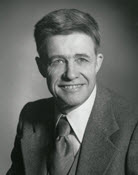
\includegraphics[scale = 1]{images/iverson.jpg}
\end{center}

\subsubsection{}

Un altro personaggio importante fu Raimondo Lullo, un filosofo, teologo e missionario catalano. Egli fu il primo a proporre un sistema di combinazione di segni per ottenere nuove conoscenze. Il suo sistema era basato su un insieme di simboli che rappresentavano le nozioni e le relazioni tra di esse. Questo sistema era chiamato \fancyglitter{Ars Magna}.
Oltre a ciò si occupò di \fancyglitter{logica combinatoria} nella sua opera \fancyglitter{Ars Combinatoria}.

\section{Leibniz}

Nasce a Lipsia il 21 Giugno 1646, si laurea in Giurisprudenza nel 1666.
I suoi primi scritti sono finalizzati al conseguimento di titoli accademici. Importante in
questo periodo è la Dissertatio de Arte Combinatoria del 1666.
Negli anni immediatamente successivi alla laurea diventa consigliere dell’Elettore di
Magonza e assume diversi incarichi politici.

\begin{center}
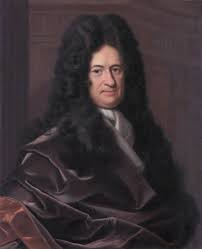
\includegraphics[scale = 0.7]{images/Leibniz.jpg}
\end{center}

Nel 1672 viene inviato a Parigi in missione diplomatica, per distogliere Luigi XIV dalla
progettata invasione dell’Olanda e invogliarlo invece alla conquista dell’Egitto.
Fallita la missione, ottiene il permesso di fermarsi a Parigi (e Londra), dove rimane per 4
anni (marzo 1672 - ottobre 1676) avendo la possibilità di conoscere la matematica e la
fisica più avanzate. Nel 1676 scopre il calcolo infinitesimale (che verrà pubblicato solo ne 1684), già
introdotto da Newton indipendentemente 10 anni prima. Nel 1705 inizierà tra i due una
polemica che finirà solo con la morte di Leibniz.
Nello stesso anno torna a Hannover come bibliotecario presso il Duca.

Tra il 1685 e il 1694: migliora la scatola di Pascal (\fancyglitter{pascalina}) per l’addizione e la sottrazione per realizzare
anche la moltiplicazione e la divisione (e l’estrazione di radice). La macchina, che opera
mediante pulegge e ruote dentate, è conservata nella biblioteca di Hannover.

\subsection{L'origine del bit}

Leibniz fece un parallelismo tra i simboli dello yin e dello yang e i numeri binari.
Le linee piene potevano essere associate al 1, mentre le linee vuote al 0.
Così facendo si ottiene un sistema di numerazione binario.

\begin{center}
    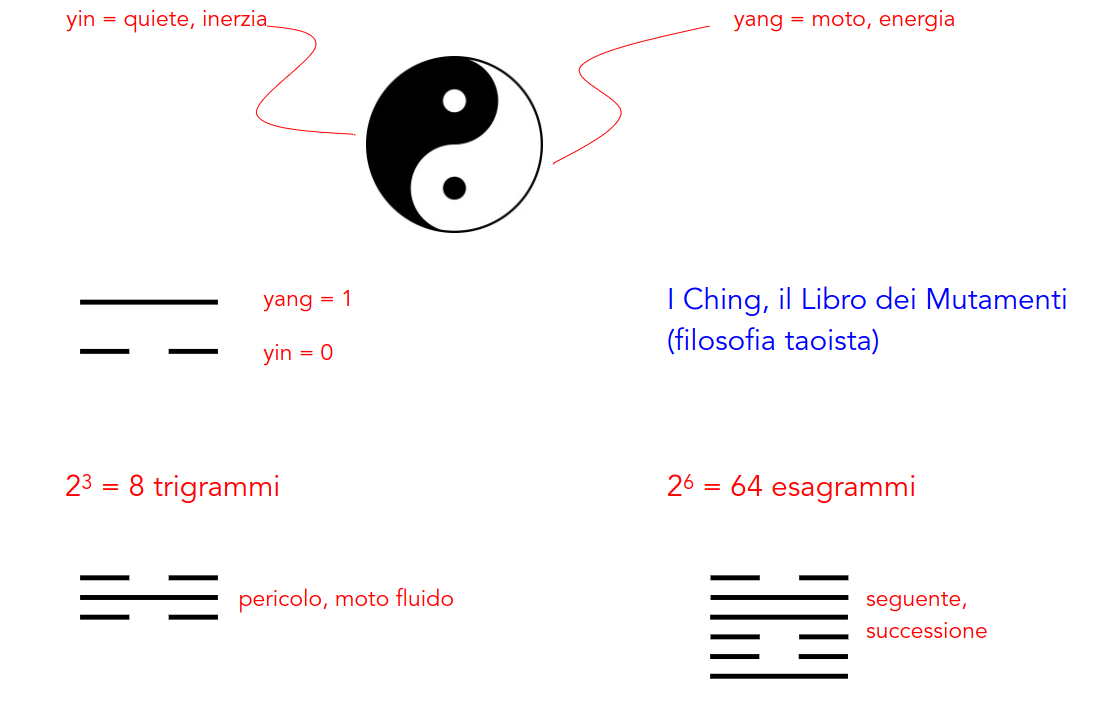
\includegraphics[scale = 0.3]{images/Origine bit.png}
\end{center}

\pagebreak

\ex{L'interpretazione di Leibniz}{
    \begin{center}
        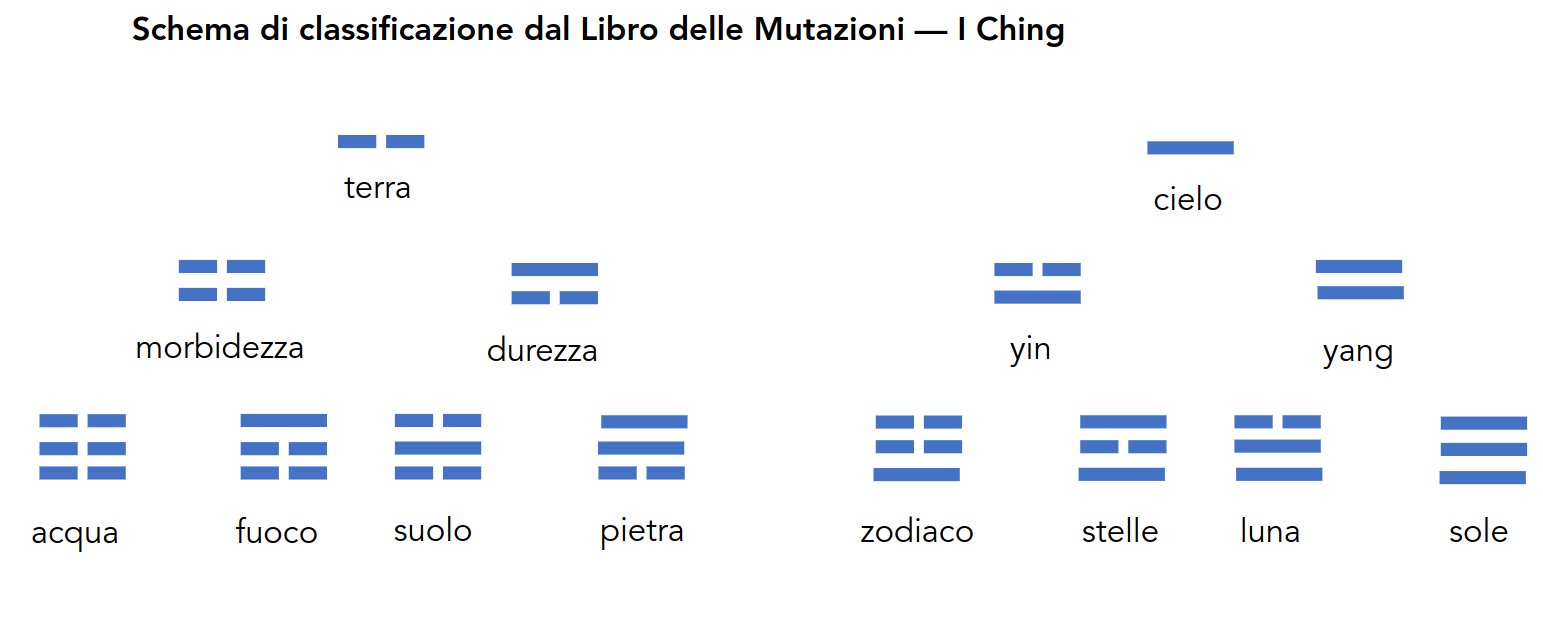
\includegraphics[scale = 0.27]{images/Bit.png}
        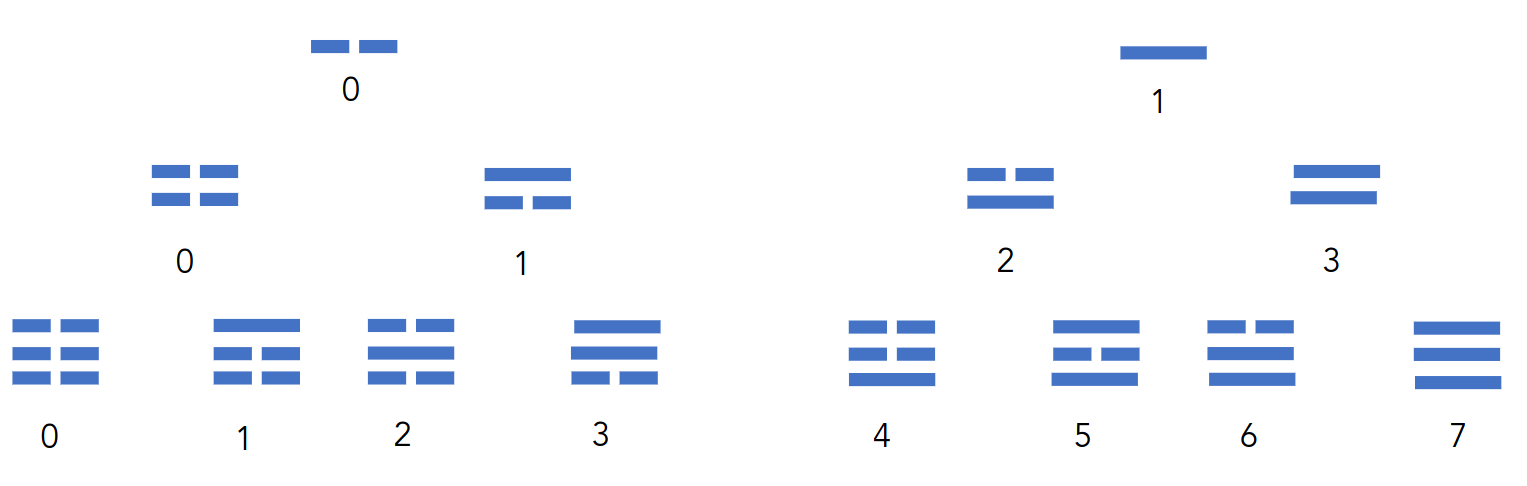
\includegraphics[scale = 0.27]{images/Associazione di Leibniz.png}
    \end{center}
}

\subsection{La caratteristica universale}

La \fancyglitter{caratteristica universale}, concepita come lingua o scrittura universale, si fonda sui seguenti principi:

\begin{itemize}
    \item [$\Rightarrow$] Le idee sono analizzabili fino a idee semplici (atomiche);
    \item [$\Rightarrow$] Le idee possono essere rappresentate da simboli;
    \item [$\Rightarrow$] Le relazioni tra idee possono essere rappresentate da simboli;
    \item [$\Rightarrow$] Le idee si combinano mediante regole.
\end{itemize}

\dfn{Caratteristica universale}{
La \newfancyglitter{caratteristica universale}\footnote{Ispirata da Lullo e dal "Lullismo", da Atanasio Kircher e da uno scrittore anonimo del 1663.} è un sistema di segni che rappresentano
nozioni e cose, ma non parole. Le connessioni tra i segni rappresentano le relazioni tra le nozioni e le cose.
Il nome di una nozione serve a:
\begin{itemize}
    \item [$\Rightarrow$] Relazionarla con altre nozioni;
    \item [$\Rightarrow$] Relazionarla con lo schema dell'universo;
    \item [$\Rightarrow$] Indicare le esperienze necessarie per la conoscenza.
\end{itemize}
}

\nt{L'apprendimento della lingua universale coincide con l'\fancyglitter{enciclopedia}. }

\subsubsection{Il calculus ratiocinator}

\dfn{Calculus ratiocinator}{Il \newfancyglitter{calculus ratiocinator} è un insieme di tecniche per manipolare i segni della caratteristica universale. Può essere considerato come un \newfancyglitter{sistema formale}. Il frammento XX offre un'idea di questo calcolo: in esso vengono trattati molti assiomi e teoremi come il principio degli indiscernibili, la simmetria, la transitività, etc.}

\subsection{La mereologia del Frammento XX}

\dfn{Mereologia}{
    La \newfancyglitter{mereologia} è la "dottrina delle parti".
}

\dfn{Principio di identità degli indiscernibili}{
    Sono identici i termini che possono essere sostituiti a vicenda
    senza alterare la verità degli enunciati in cui compaiono. Si scrive A = B 
    quando A e B sono identici.
    \begin{itemize}
        \item [$\Rightarrow$] $B + N = L$ significa che B e N compongono L,
        cioè che B è parte di L;
        \item [$\Rightarrow$] $A\leq B$ significa che A è parte di B.
    \end{itemize}
}

\thm{Simmetria}{
    Se $A = B$ allora $B = A$.
}

\thm{Transitività}{
    Se $A = B$ e $B = C$ allora $A = C$.
}

\thm{}{
    Se $A + B = B$ allora $A \leq B$.
}

\thm{}{
    Se $A = B$ allora $A + L = B + L$.
}

\section{Ulteriori sviluppi}

\subsection{Peano e i numeri naturali}

Peano nacque a Cuneo il 27 agosto 1858. Si laureò in matematica nel 1880 e divenne professore di analisi matematica a Torino nel 1890. Nel 1889 pubblicò i suoi famosi \newfancyglitter{Principi di aritmetica}, in cui formulò un sistema assiomatico per i numeri naturali.

\begin{center}
    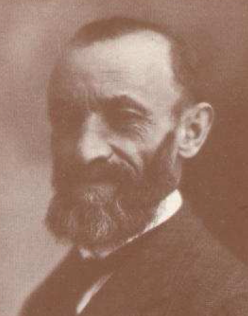
\includegraphics[scale = 0.35]{images/Peano.png}
\end{center}

\dfn{Principi di aritmetica}{
    I \newfancyglitter{Principi di aritmetica} sono un insieme
    di assiomi che definiscono i numeri naturali.
}

\subsection{Hilbert e lo Entscheidungsproblem}

Hilbert fu un matematico tedesco nato a Königsberg il 23 gennaio 1862. Egli fu uno dei più grandi matematici del XX secolo e fu uno dei fondatori della logica matematica.
Nel 1928, insieme ad Ackermann, pubblicò il libro \fancyglitter{Grundzüge der theoretischen Logik} in cui venne enunciato il \fancyglitter{problema della decisione} (
    o \fancyglitter{Entscheidungsproblem}).

\dfn{Entscheidungsproblem}{
    L'\newfancyglitter{Entscheidungsproblem} è un problema che consiste nel trovare una procedura che consente di decidere la validità di una data espressione logica con un 
    numero finito di operazioni.
}

\section{La logica matematica}

\nt{Sono trattati più in dettaglio nel corso "Metodi formali dell'Informatica" e, in
misura minore, nel corso di "Linguaggi e paradigmi di programmazione".}

\subsection{Sistemi formali}

\dfn{Sistema formale}{
    In un \newfancyglitter{sistema formale} si definiscono:
    \begin{itemize}
        \item [$\Rightarrow$] \newfancyglitter{Oggetti}, che sono tutti i termini costruibili a partire 
        da atomi mediante operazioni;
        \item [$\Rightarrow$] \newfancyglitter{Proposizioni}, della forma $P(a_1, ..., a_n)$ dove
        $P$ è un \newfancyglitter{predicato} e $a_k$ sono termini;
        \item [$\Rightarrow$] \newfancyglitter{Regole di inferenza}, che permettono di dedurre nuove proposizioni.
        La conclusione di una regola di inferenza senza premesse è un'\newfancyglitter{assioma}.
    \end{itemize}

    $$\frac{A_1 \:\:\:\:\:\:\:\:\:...\:\:\:\:\:\:\:\:\: A_v}{A}$$
}

\qs{}{Come si usano le regole di inferenza?}

\paragraph{Risposta:} Per costruire derivazioni: 

\begin{figure}[h]
    \centering
    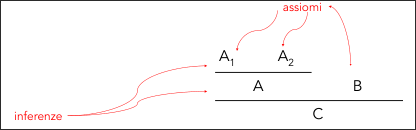
\includegraphics[scale = 0.55]{images/Inferenza.png}
    \caption{Derivazione.}
\end{figure}

\ex{Numeri naturali}{
    \begin{itemize}
        \item [$\Rightarrow$] \fancyglitter{Oggetti}: un atomo 0, un'operazione S, con un solo argomento;
        \item [$\Rightarrow$] \fancyglitter{Proposizioni}: un predicato Num con un solo argomento;
        \item [$\Rightarrow$] \fancyglitter{Regole di inferenza}: $\frac{}{\text{Num\{0\}}}$ e 
        $\frac{\text{Num\{n\}}}{\text{Num\{S(n)\}}}$.
    \end{itemize}
}

\ex{Grammatiche formali}{
    \begin{center}
        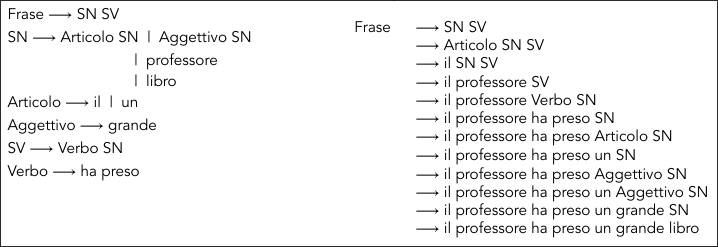
\includegraphics[scale = 0.35]{images/Gram.png}
    \end{center}
}

\subsection{Confronto tra logica e informatica}

\paragraph{Logica:}

\begin{itemize}
    \item [$\Rightarrow$] Si studiano modelli di processi deduttivi;
    \item [$\Rightarrow$] Si studiano modelli di ragionamento;
    \item [$\Rightarrow$] Operatori modali.
\end{itemize}

\paragraph{Informatica:}

\begin{itemize}
    \item [$\Rightarrow$] Si studiano modelli di processi trasformazionali;
    \item [$\Rightarrow$] Si studiano modelli di calcolo (sequenziali, paralleli, distribuiti).
\end{itemize}


\subsection{Kleene e le funzioni ricorsive}

Nel 1981 Stephen Cole Kleene, matematico e logico statunitense,
pubblicò l'articolo "\fancyglitter{Origins of recursive function theory}" in cui
descrisse l'attività di ricerca svolta da alcuni matematici
e logici negli anni '30. In particolare, Kleene descrisse
una serie di lezioni di G\"odel tenute nel 1934 a Princeton
sullo sviluppo di definizioni ricorsive primitive di funzioni 
numeriche. Lo \fancyglitter{schema di ricorsione primitiva} permette di
definire una funzione di numeri naturali f(\textbf{x}, n) a partire da funzioni 
predefinite b(\textbf{x}) e h(\textbf{x}, n, m) mediante lo schema:

$$f(x, 0) = b(x)$$

$$f(x, n + 1) = h(x, n , f(x, n))$$
\subsubsection*{}
Inoltre si ha la composizione:

$$f(x) = h(g_1(x), \cdot\cdot\cdot, g_k(x))$$

\subsubsection{}

G\"odel usava la nozione di \fancyglitter{sistema matematico formale} basata
sulla nozione informale di \fancyglitter{regola costruttiva} la cui
applicazione si basava su una \fancyglitter{procedura finita} del tipo
necessario per calcolare funzioni definite mediante ricorsioni generali.
\subsubsection{}
Nasce il problema della caratterizzazione delle ricorsioni ammissibili.
Kleene aggiunse un \fancyglitter{operatore di ricerca} non limitato
che dato un predicato P(x, y) restituisce il valore minimo che soddisfa
il predicato. 
Nel 1938, Kleene ammise la possibilità di definire funzioni
parziali.

\section{Curry e la logica combinatoria}

Nel 1927, Haskell Brooks Curry, matematico e logico statunitense,
riscopri la nozione di \fancyglitter{combinatore} (introdotta da
Moses Sch\"onfinkel nel 1920).

\dfn{Combinatore}{
    Un \newfancyglitter{combinatore} è una funzione senza variabili libere.
}

\nt{I sistemi di combinatori attuali usano K e S come combinatori,
perché sono sufficienti a generare tutti gli altri combinatori.}

\ex{Combinatori}{
    \begin{itemize}
        \item [$\Rightarrow$] K(x, y) = x;
        \item [$\Rightarrow$] S(x, y, z) = x(z)(y(z)).;
        \item [$\Rightarrow$] B(x, y, z) = x(y(z));
        \item [$\Rightarrow$] C(x, y, z) = x(z)(y);
        \item [$\Rightarrow$] W(x, y) = x(y)(y).
        \item [$\Rightarrow$] I(x) = x.
    \end{itemize}
}

\subsubsection*{}

Inoltre riprende anche la possibilità di trattare funzioni a più argomenti
come funzioni a un solo argomento che verrà chiamata \fancyglitter{curryficazione}.

$$f(x, y) = f'(x)(y)$$

\subsubsection*{}

Nello stesso tempo, Alonzo Church, sviluppa il \fancyglitter{lambda calcolo}\footnote{Visto approfonditamente nei corsi 
"Metodi formali dell'informatica" e "Linguaggi e paradigmi di programmazione, per cui in questi appunti non andrò
in dettaglio dato che esula gli obiettivi del corso.}.

\dfn{Lambda calcolo}{
    Il \newfancyglitter{lambda calcolo} è un sistema formale per la definizione di funzioni
    intese come regole di corrispondenza. $\lambda x.M$ descrive la regola che assegna
    a un argomento $x$ il valore $M$.
}

\subsection{Paradosso di Russell e combinatori}

$$WS(BWB) = Y = \lambda x.(\lambda z.x(zz)) (\lambda z.x(zz))$$

\nt{Si tratta del combinatore di punto fisso.
Permette di definire funzioni ricorsive.}

\dfn{Paradosso di Russell}{

    $$(\lambda x.(\lambda z.x(zz)) (\lambda z.x(zz))) \neg = 
     (\lambda z.\neg(zz)) (\lambda z.\neg(zz))$$

    In cui $\{z | \neg (z \in z)\} \in \{z | \neg (z \in z)\}$.
    Ciò vuol dire che qualcosa appartiene a se stesso, ma
    non può appartenere a se stesso.

}

\section{L'analisi dei processi di calcolo di Turing}

Nel paragrafo 9 del suo articolo del 1936, Turing introduce
il comportamento di un \fancyglitter{computor}. Lo esemplifica con un
foglio di carta che viene astratto come un "nastro infinito" suddiviso in
caselle (quadratini):
\begin{itemize}
    \item [$\Rightarrow$] Il numero di simboli che si possono stampare è finito,
    perché se ci fossero infiniti simboli ci si potrebbe confondere\footnote{Un po'
    come il fatto che molti caratteri Unicode non possono essere usati nei
    nomi dei siti web in quanto troppo "simili".};
    \item [$\Rightarrow$] Il comportamento è determinato dallo stato mentale
    e dal simbolo osservato, c'è un limite alla percezione delle caselle per lo stesso
    motivo di prima;
    \item [$\Rightarrow$] Le operazioni sono elementari, cioè non possono essere
    ulteriormente scomposte. Esse consistono in cambiamenti di stato mentale e  
    del simbolo osservato\footnote{Un solo simbolo viene alterato.}.
\end{itemize}

\begin{figure}[h]
    \centering
    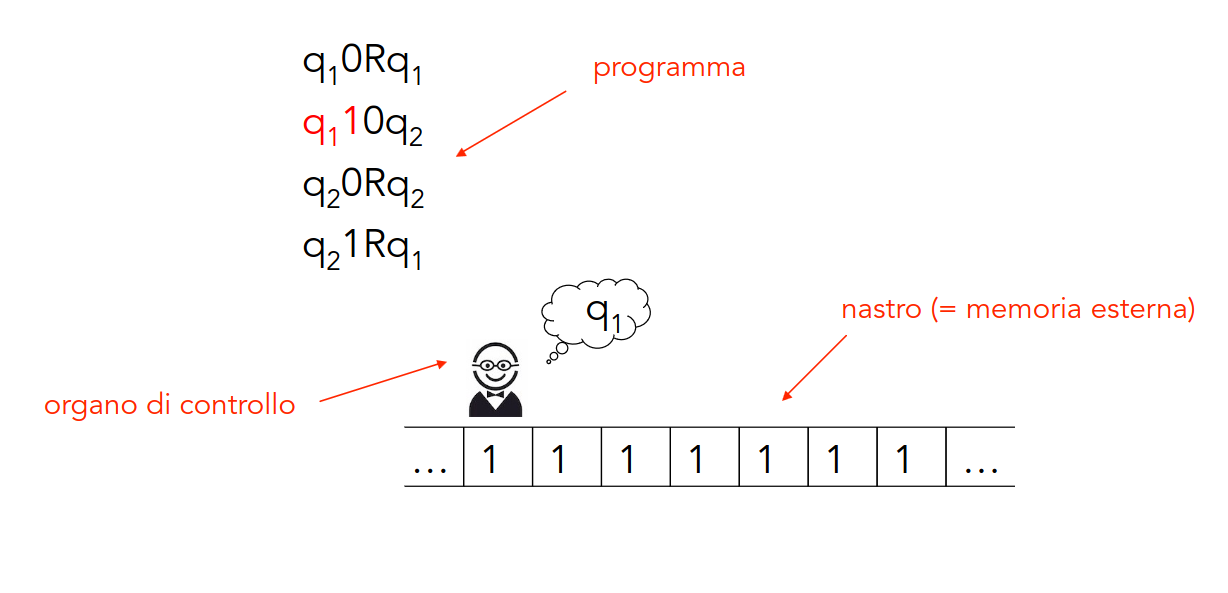
\includegraphics[scale = 0.35]{images/Turing.png}
    \caption{Macchine di Turing come Computer.}
\end{figure}

\dfn{Macchina universale}{
    Una \newfancyglitter{macchina universale} ($U$) è una macchina di Turing
    che può simulare il comportamento di qualsiasi altra macchina di Turing ($M$)
    dato il suo programma ($I_M$) per ogni dato $x$:

    $$U(I_M, x) = M(x)$$

    È possibile che $U$ sia più complessa di $M$. In informatica, il
    programma di $U$ è chiamato \newfancyglitter{interprete}. 

    }

    \nt{Questo risultato suggerirà a von Neumann la possibilità di
    automi che generano automi di pari o maggiore complessità.}


\subsection{Non tutte le funzioni sono calcolabili da una macchina di Turing}

Per dimostare che non tutte le funzioni sono calcolabili da una macchina di Turing  si può
utilizzare la \fancyglitter{diagonalizzazione di Cantor}\footnote{Visto nel corso "Matematica discreta".}:
\begin{itemize}
    \item [$\Rightarrow$] Si immagina di poter numerare le funzioni da $\bbN$ in $\bbN$;
    \item [$\Rightarrow$] Si considera una funzione da $\bbN$ in $\{0,1\}^\bbN$;
    \item [$\Rightarrow$] Questo elenco può essere visto come una tabella;
    \item [$\Rightarrow$] Si vuole dimostrare che esiste una sequenza che non è in questa tabella;
    \item [$\Rightarrow$] Si prende la diagonale, che interseca tutte le righe in un punto;
    \item [$\Rightarrow$] Si cambiano tutti i valori della diagonale (0 diventa 1 e viceversa);
    \item [$\Rightarrow$] La diagonale trasformata può essere una riga dell'originale?
    \item [$\Rightarrow$] No, perché differisce da ogni riga in almeno un punto.
\end{itemize}

\begin{figure}[h]
    \centering
    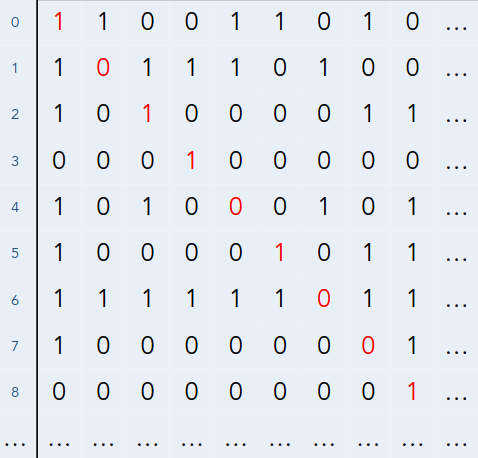
\includegraphics[scale = 0.38]{images/Diagonalizzazione.png}
    \caption{Diagonalizzazione di Cantor.}
\end{figure}

\begin{figure}[h]
    \centering
    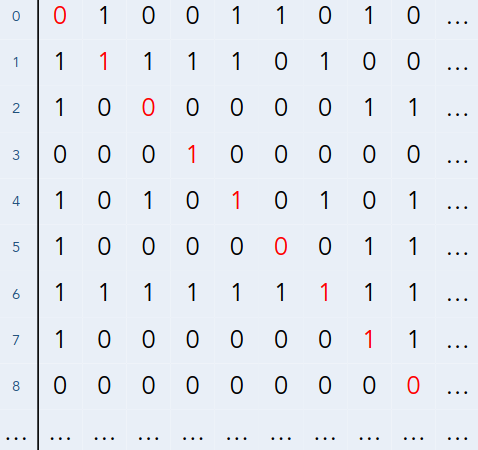
\includegraphics[scale = 0.38]{images/Diagonalizzazione 2.png}
    \caption{Diagonalizzazione di Cantor, inversione della diagonale.}
\end{figure}

\cor{Problemi indecidibili}{
    Non esiste una macchina di Turing $M$ che, operando su un nastro che contiene:
    \begin{itemize}
        \item [$\Rightarrow$] La descrizione di una qualsiasi macchina di Turing $T$;
        \item [$\Rightarrow$] Un input $x$.
    \end{itemize}
    termina sempre i suoi calcoli scrivendo sul nastro il valore $M(T, x)$ dove:
    \begin{itemize}
        \item [$\Rightarrow$] $M(T, x) = 1$ se $T(x)$ termina;
        \item [$\Rightarrow$] $M(T, x) = 0$ se $T(x)$ non termina.
    \end{itemize}
}
\nt{Il problema della fermata è indecidibile.}

\section{Von Neumann: il Computer come Organismo Artificiale}

Von Neumann, matematico e fisico ungherese\footnote{Già visto
nella prima parte del corso.}, fu influenzato dalle idee di
McCulloch e Pitts\footnote{
    \textit{A logical calculus of the ideas immanent in nervous activity}.
}, che avevano definito un modello di neurone
le cui reti potevano essere caratterizzate come \fancyglitter{automi finiti}\footnote{Notato da Kleene nel 1951}.

\begin{figure}[h]
    \centering
    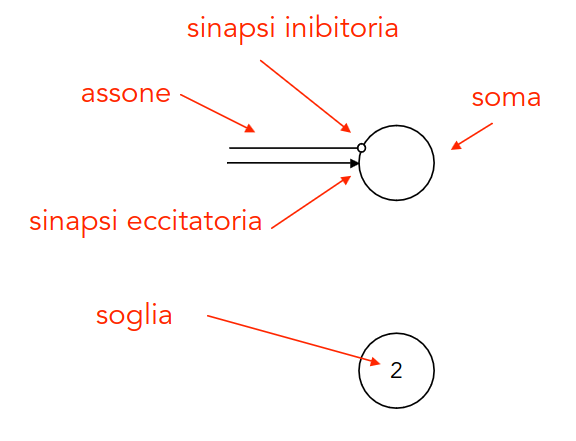
\includegraphics[scale = 0.25]{images/McCulloch-Pitts.png}
    \caption{Il neurone di McCulloch e Pitts.}
\end{figure}

\subsubsection{}

Nel 1945, von Neumann pubblicò il "First Draft of a Report on the EDVAC" in cui
descriveva gli elementi di un calcolatore in termini "biologici" utilizzando
il modello di McCulloch e Pitts:

\begin{itemize}
    \item [$\Rightarrow$] \fancyglitter{CPU}: neuroni di associazione;
    \item [$\Rightarrow$] \fancyglitter{Input}: neuroni sensoriali;
    \item [$\Rightarrow$] \fancyglitter{Output}: neuroni motori.
\end{itemize}

\subsubsection{}

L'obiettivo di von Neumann era quello di \fancyglitter{unificare}, tramite una
teoria generale degli automi, il lavoro di Turing sulle macchine teoriche,
il lavoro di McCulloch e Pitts sui neuroni e il lavoro di Shannon sulla
teoria dell'informazione\footnote{Si vedrà nel prossimo capitolo.}.

\nt{Questo tentativo verrà criticato dai neurofisiologi perché
tentava di descrivere computer e cervello assiomatizzando il comportamento
di \fancyglitter{scatole nere}.}

\subsection{Automi cellulari}

Negli anni '40, a Los Alamos, von Neumann e Ulam ebbero l'idea di
automi che operino su una griglia di celle infinita (bidirezionale).
Ogni cella ha un proprio stato e lo stato di una cella in un'istante $T$
dipende dallo stato delle celle adiacenti in un istante $T - 1$. Il modello
di von Neumann e Ulam aveva 29 stati.

\clm{}{}{
    Da notare che la nozione di \fancyglitter{celle adiacenti} è relativa:
    per von Neumann erano solo 4 (nord, sud, est, ovest), mentre per Moore
    erano 8 (aggiungeva anche le diagonali). Oltre a questo esistono altri modelli con
    celle esagonali e con forme diverse.
}

\begin{figure}[h]
    \centering
    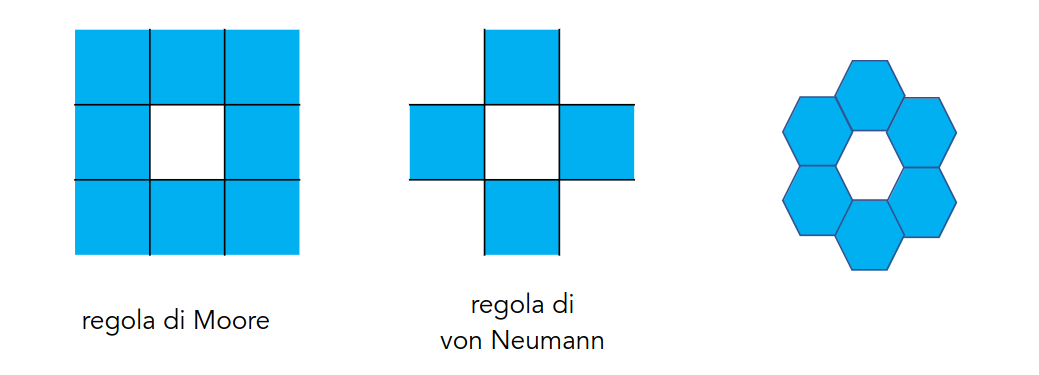
\includegraphics[scale = 0.3]{images/Automi cellulari.png}
    \caption{Ci sono differenti versioni.}
\end{figure}

\paragraph{Per von Neumann c'erano due modi di descrivere gli automi cellulari:}

\begin{itemize}
    \item [$\Rightarrow$] \fancyglitter{McCulloch-Pitts (modo sintetico)}: strutture
    costruite a partire da elementi più semplici. Bisogna solo definire gli elementi e le loro connessioni (può essere complesso);
    \item [$\Rightarrow$] \fancyglitter{Turing (modo integrale)}: si descrive, tramite assiomi, l'intero automa senza descrivere
    gli elementi da cui è composto, ma solo il loro comportamento.
\end{itemize}

\begin{figure}[h]
    \centering
    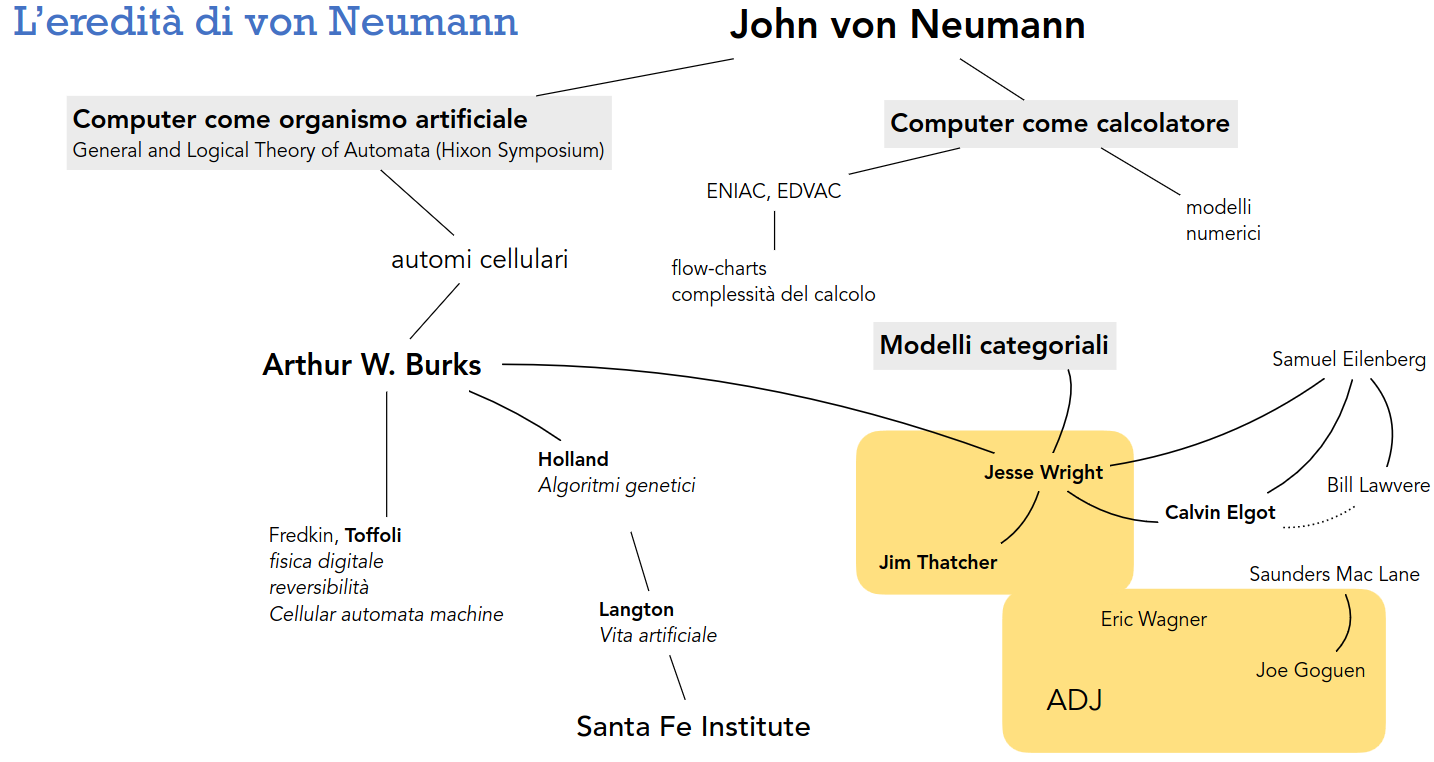
\includegraphics[scale = 0.33]{images/V1.png}
    \caption{Sommario.}
\end{figure}

\subsection{La Vita Artificiale secondo Conway (Game of Life)}

\dfn{Game of Life}{
    Il \newfancyglitter{Game of Life} è un automa cellulare ideato da John Conway nel 1970.
    Si basa su una griglia bidimensionale di celle quadrate, ognuna delle quali può essere
    in uno di due stati: vivo o morto. Le celle comunicano con le otto celle adiacenti.
    È un gioco a zero giocatori, cioè il suo sviluppo è determinato solo dallo stato iniziale.
}

\cor{Regole}{
    Le regole sono le seguenti:
    \begin{itemize}
        \item [$\Rightarrow$] Una cella morta con esattamente tre celle vive adiacenti diventa viva;
        \item [$\Rightarrow$] Una cella viva con due o tre celle vive adiacenti rimane viva;
        \item [$\Rightarrow$] In tutti gli altri casi la cella muore.
    \end{itemize}
}

\begin{figure}[h]
    \centering
    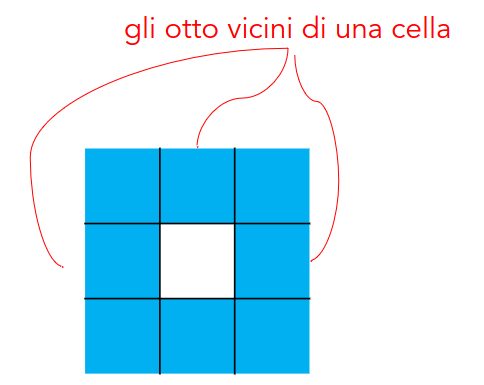
\includegraphics[scale = 0.3]{images/Conway.png}
    \caption{Game of Life.}
\end{figure}

\nt{Una configurazione famosa è il \fancyglitter{glider} (aliante), che si muove
nella griglia.}

\begin{figure}[h]
    \centering
    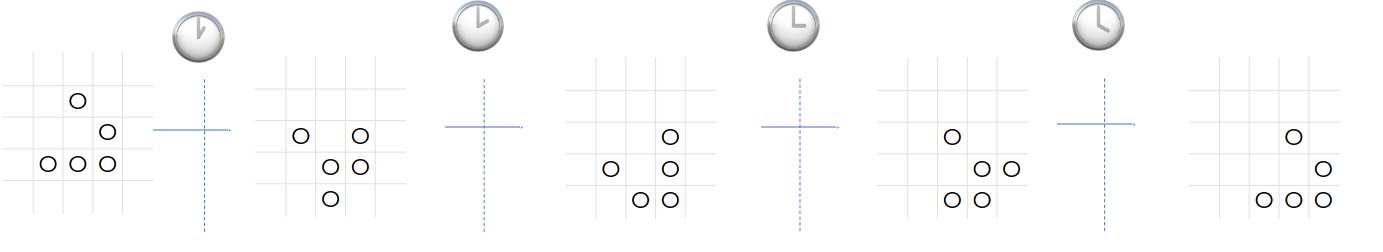
\includegraphics[scale = 0.3]{images/Glider.png}
    \caption{Glider.}
\end{figure}
